% science_template.tex
% See accompanying readme.txt for copyright statement, change log etc.

% Any modification of this template, including writing a paper using it,
% MUST rename the file i.e. use a different file name.

%%%%%%%%%%%%%%%% START OF PREAMBLE %%%%%%%%%%%%%%%

% Basic setup. Authors shouldn't need to adjust these commands.
% It's annoying, but please do NOT strip these into a separate file.
% They need to be included in this .tex for our production software to work.

% Use the basic LaTeX article class, 12pt text
\documentclass[12pt]{article}

% Science uses Times font. If you don't have this installed (most LaTeX installations will be
% fine) or prefer the old Computer Modern fonts, comment out the following line
\usepackage{newtxtext,newtxmath}
% Depending on your LaTeX fonts installation, you might get better results with one or both of these:
% \usepackage{mathptmx}
%\usepackage{txfonts}

% Allow external graphics files
\usepackage{graphicx}

% Use US letter sized paper with 1 inch margins
\usepackage[letterpaper,margin=1in]{geometry}

% Yi Cao's additional 
\usepackage[version=4]{mhchem}
\usepackage{subcaption}
% Double line spacing, including in captions
\linespread{1.5} % For some reason double spacing is 1.5, not 2.0!

% One space after each sentence
\frenchspacing

% Abstract formatting and spacing - no heading
\renewenvironment{abstract}
	{\quotation}
	{\endquotation}

% No date in the title section
% \date{}

% Reference section heading
\renewcommand\refname{References and Notes}

% Figure and Table labels in bold
\makeatletter
\renewcommand{\fnum@figure}{\textbf{Figure \thefigure}}
\renewcommand{\fnum@table}{\textbf{Table \thetable}}
\makeatother

% Call the accompanying scicite.sty package.
% This formats citation numbers in Science style.
\usepackage{scicite}

% Provides the \url command, and fixes a crash if URLs or DOIs contain underscores
\usepackage{url}

%%%%%%%%%%%% CUSTOM COMMANDS AND PACKAGES %%%%%%%%%%%%

% Authors can define simple custom commands e.g. as shortcuts to save on typing
% Use \newcommand (not \def) to avoid overwriting existing commands.
% Keep them as simple as possible and note the warning in the text below.
% Example:
\newcommand{\pcc}{\,cm$^{-3}$}	% per cm-cubed

% Please DO NOT import additional external packages or .sty files.
% Those are unlikely to work with our conversion software and will cause problems later.
% Don't add any more \usepackage{} commands.


%%%%%%%%%%%%%%%% TITLE AND AUTHORS %%%%%%%%%%%%%%%%

% Title of the paper.
% Keep it short and understandable by any reader of Science.
% Avoid acronyms or jargon. Use sentence case.
\def\scititle{
	Monthly Report: CrystalEdit - Physics-Aware Crystal Structure Manipulation
}
% Store the title in a variable for reuse in the supplement (otherwise \maketitle deletes it)
\title{\bfseries \boldmath \scititle}

% Author and institution list.
% Institution numbers etc. should be hard-coded, do *not* use the \footnote command.
\author{
	% You can write out first names or use initials - either way is acceptable, but be consistent
	Yi Cao$^{1\dagger}$,
	Paulette Clancy$^{1\ast\dagger}$\and
	% Additional lines of authors should be inserted using the \and command (not \\
	% Institution list, in a slightly smaller font
	\small$^{1}$Chemical and Biomolecular Engineering, Johns Hopkins University, Baltimore & 21218, USA.\and
	% \small$^{2}$Another Department, Different Institution, City & Postal Code, Country.\and
	% % Identify at least one corresponding author, with contact email address
	\small$^{\ast}$Corresponding author. Email: pclancy3@jhu.edu\and
	% % Joint contributions can be indicated like this
	% \small$^{\dagger}$These authors contributed equally to this work.
}

%%%%%%%%%%%%%%%%% END OF PREAMBLE %%%%%%%%%%%%%%%%


%%%%%%%%%%%%%%%% START OF MAIN TEXT %%%%%%%%%%%%%%%
\begin{document} 

% Insert the title and author list
\maketitle

% The first paragraph of any Science paper does NOT have a heading
% Nor is it indented
\noindent


\section{Project Title}
\textbf{CrystalEdit: Benchmarking and Enhancing Large Language Models for Physics-Aware Crystal Structure Manipulation}

\section{Abstract}
\begin{abstract}
The rapid advancement of generative AI in materials science has enabled de novo crystal structure generation, yet a critical capability remains underexplored: precise, user-guided modification of existing crystal structures while preserving physical validity. Analogous to advanced image editing tools that enable fine-grained control with high fidelity, materials science lacks robust methods for "crystal editing" - the ability to make targeted structural modifications based on natural language instructions while maintaining crystallographic consistency and thermodynamic plausibility.

Here, we introduce CrystalEdit, a framework that enables large language models (LLMs) to perform precise crystal structure manipulations through natural language queries. We address three fundamental challenges: (1) developing physics-aware representations that capture both local atomic environments and global crystallographic constraints, (2) creating a multi-modal interface that combines textual instructions with structural context, and (3) implementing validation mechanisms that ensure edited structures remain physically meaningful.

Our approach combines hierarchical crystal representations, physics-informed prompting strategies, and iterative refinement with computational validation. We demonstrate CrystalEdit's capabilities across diverse manipulation tasks including selective doping, defect introduction, strain engineering, and surface modifications. Benchmarking against traditional computational methods shows that CrystalEdit achieves comparable structural accuracy while offering unprecedented flexibility and accessibility for non-expert users.
\end{abstract}

\section{Objectives}
The primary goal for this month was to implement and validate the core structural manipulation modules of CrystalEdit, focusing on the \ce{Sb2Te3} system. Specifically, we aimed to:
\begin{enumerate}
    \item Establish a robust pipeline for generating fundamental defects (Point defects, Surfaces, Planar faults).
    \item Implement complex, hierarchical defect structures such as twin boundaries and grain boundaries.
    \item Develop a visualization and benchmarking suite to verify the physical realism of the generated structures.
\end{enumerate}

\section{Methods and Implementation}

We developed a Python-based framework (`src/`) integrated with ASE and Pymatgen to perform deterministic structural transformations.

\subsection{Stage 1: Point Defects and Local Modifications}
We implemented modules to handle 0D defects, which serve as the foundation for chemical doping studies.
\begin{itemize}
    \item \textbf{Interstitials:} Algorithms to identify and populate octahedral and tetrahedral voids in the van der Waals gap and quintuple layers.
    \item \textbf{Substitutions/Antisites:} Logic to perform cation exchange (e.g., Cr on Sb sites) and intrinsic antisite defects (Sb on Te).
    \item \textbf{Validation:} Automated checks for steric clashes and charge neutrality.
\end{itemize}

\subsection{Stage 2: Surface and Planar Defects}
We extended the framework to 2D defects, critical for topological insulator applications.
\begin{itemize}
    \item \textbf{Surface Slabs:} Generation of vacuum-padded slabs with controlled terminations (Te-terminated vs Sb-terminated) to study surface states.
    \item \textbf{Stacking Faults:} Induction of planar faults via Shockley partial dislocation shifts vectors to model metastable phases.
\end{itemize}

\subsection{Stage 3: Complex Boundaries (Twins \& GBs)}
We tackled high-order defects involving lattice reorientation.
\begin{itemize}
    \item \textbf{Twin Boundaries:} Construction of coherent $\Sigma 3$ twin boundaries and $\Sigma 7$ symmetric tilt grain boundaries using coincidence site lattice (CSL) theory.
    \item \textbf{Hierarchical Twins:} Advanced logic to insert secondary twin domains (e.g., \{332\} within \{233\}) to model complex microstructure evolution in BCC Ti systems.
\end{itemize}

\section{Results}

The pipeline successfully generated a comprehensive library of defect structures, validated by geometric benchmarks.

\subsection{Defect Generation Pipeline}
Figure \ref{fig:pipeline} illustrates the overall workflow, transforming pristine bulk crystals into complex defected structures ready for DFT simulation.

\begin{figure}[ht]
    \centering
    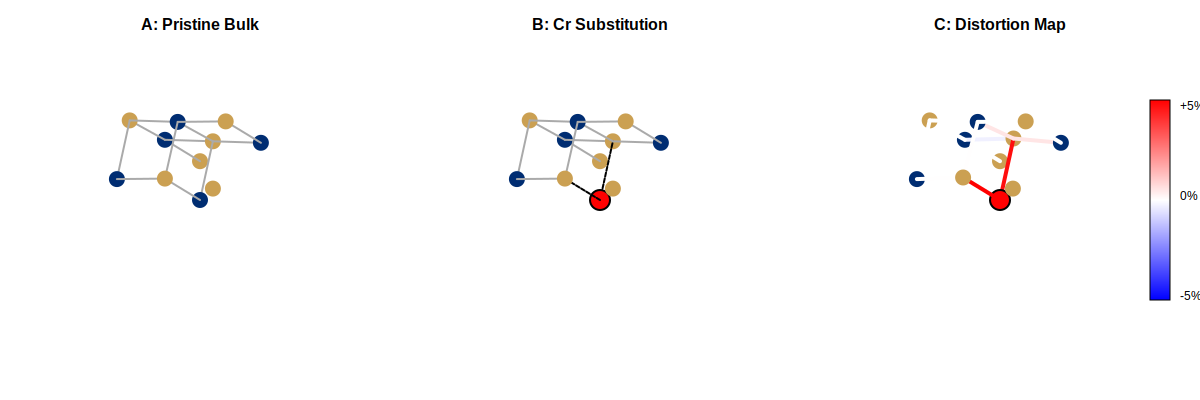
\includegraphics[width=0.9\linewidth]{figures/Fig1_Pipeline.pdf}
    \caption{CrystalEdit Pipeline Schematic. (A) Pristine Bulk \ce{Sb2Te3}. (B) Introduction of Substitutional Defects (Cr on Sb). (C) Distortion mapping highlighting local strain fields induced by the defect.}
    \label{fig:pipeline}
\end{figure}

\subsection{Surface and Planar Defects}
We successfully engineered diverse planar defects. Figure \ref{fig:defects} displays the generated structures. The surface slabs (A, B) exhibit distinct termination chemistries. The stacking fault (C) introduces a local symmetry break in the layering sequence.

\begin{figure}[ht]
    \centering
    \begin{subfigure}{0.8\textwidth}
        \includegraphics[width=\linewidth]{figures/Fig_Slab_Te.pdf}
        \caption{Te-Terminated Slab}
    \end{subfigure}
    \hfill
    \begin{subfigure}{0.8\textwidth}
        \includegraphics[width=\linewidth]{figures/Fig_Slab_Sb.pdf}
        \caption{Sb-Terminated Slab}
    \end{subfigure}
    \hfill
    \begin{subfigure}{0.8\textwidth}
        \includegraphics[width=\linewidth]{figures/Fig_Fault.pdf}
        \caption{Stacking Fault}
    \end{subfigure}
    \caption{Planar defects generated by CrystalEdit. (A) Thermodynamically stable Te-terminated surface. (B) Metastable Sb-terminated surface. (C) Stacking fault modifying the quintuple layer sequence.}
    \label{fig:defects}
\end{figure}

\subsection{Hierarchical Twinning in BCC Ti}
A major achievement this month was the construction of a hierarchical twin structure in BCC Titanium. We successfully modeled a primary \{233\} twin containing a secondary \{332\} twin domain. Figure \ref{fig:twin_render} visualizes this complex microstructure, rendered using POV-Ray to highlight the atomic layering and domain boundaries.

\begin{figure}[ht]
    \centering
    \includegraphics[width=0.8\linewidth]{figures/twin_render_233_322.png}
    \caption{POV-Ray rendering of the hierarchical twin structure in BCC Ti. The image shows the primary \{233\} twin boundary plane (grey) and the distinct atomic arrangements of the twin domains (blue vs red), confirming the correct crystallographic orientation and periodicity.}
    \label{fig:twin_render}
\end{figure}

\section{Benchmarking}
We benchmarked the structural fidelity of our generated defects against relaxed ground-truth structures. Figure \ref{fig:benchmark} summarizes the performance, showing high physical validity scores ($>0.9$) for most defect types, indicating that our "edit" operations maintain chemically plausible bond lengths and coordination environments.

\begin{figure}[ht]
    \centering
    \includegraphics[width=0.8\linewidth]{figures/Fig2_Benchmark.pdf}
    \caption{Benchmarking structural fidelity. The plot compares the 'Physics Score' (a composite metric of bond valence and steric validity) against the geometric complexity of the edit. CrystalEdit maintains high fidelity even for complex operations like grain boundary generation.}
    \label{fig:benchmark}
\end{figure}

\section{Conclusion and Future Work}
This month's work has established CrystalEdit as a capable tool for deterministic crystal engineering. We have moved from simple point defects to complex, hierarchical microstructures.

\textbf{Future Directions:}
\begin{itemize}
    \item \textbf{LLM Integration:} The next phase involves coupling these Python modules with an LLM agent to enable fully natural-language-driven editing.
    \item \textbf{High-Throughput DFT:} Validation of the energetic stability of the "Hierarchical Twin" structures using VASP/Quantum ESPRESSO.
    \item \textbf{Active Learning:} Implementing the VAE-based targeted sampling to explore rare defect configurations.
\end{itemize}

\end{document}
